\documentclass[tikz, border=10pt]{standalone}
\usepackage{pgfplots}
\pgfplotsset{compat=1.18}
\usepgfplotslibrary{groupplots}

\begin{document}

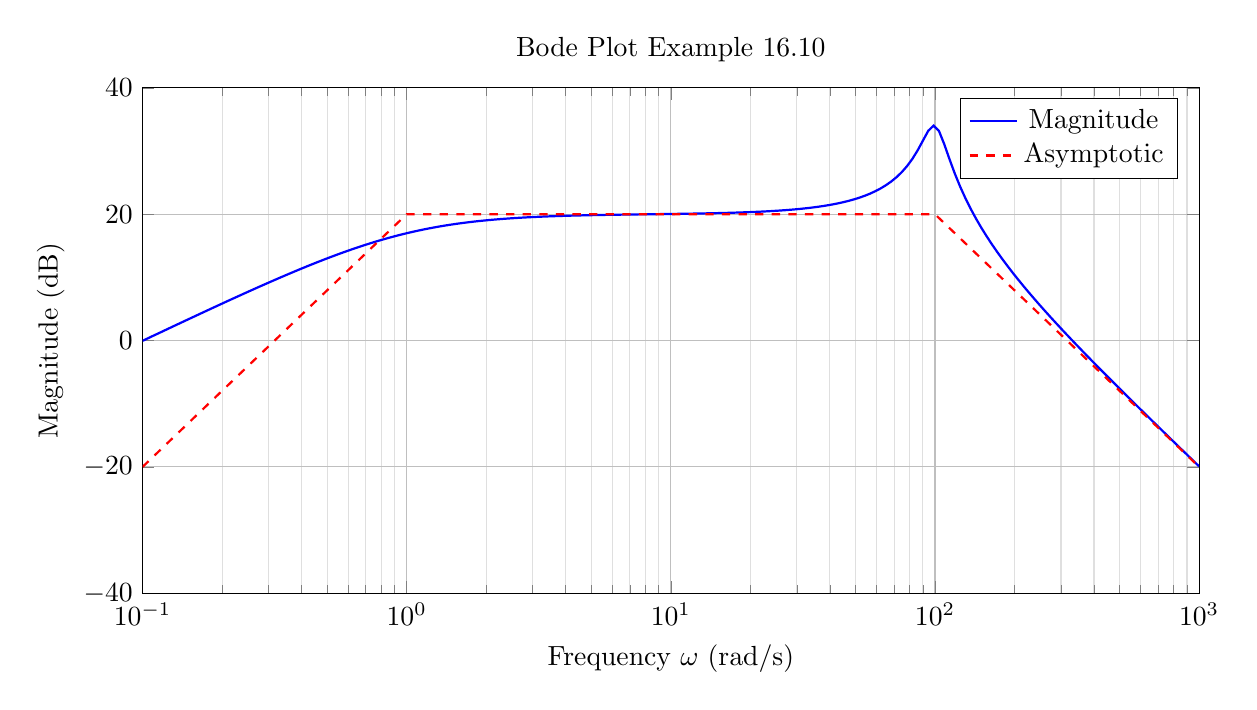
\begin{tikzpicture}
    \begin{semilogxaxis}[
        width=15cm, height=8cm,
        title={Bode Plot Example 16.10},
        xlabel={Frequency $\omega$ (rad/s)},
        ylabel={Magnitude (dB)},
        grid=both,
        xmin=0.1, xmax=1000,
        ymin=-40, ymax=40,
        minor grid style={gray!25},
        major grid style={gray!50},
    ]
    % H(s) = 10s / [ (1+s) (1 + 0.2s/100 + (s/100)^2) ] -- approximate coefficients
    % Let's plot the asymptotic approximation for Example 16.10
    % H(s) = 10s / [ (1+s)(1 + 0.002s + 0.0001s^2) ] ?
    % Detailed problem statement implies: H(s) = 10s / (1+s)(1 + 2(0.1)(s/100) + (s/100)^2)
    % Poles at 1 and 100(complex). Zero at origin.

    % Magnitude Calculation:
    % |H(jw)| = |10(jw)| / |(1+jw)| / |1 + j(0.2)(w/100) - (w/100)^2|
    % |H(jw)| = 10w / ( sqrt(1+w^2) * sqrt( (1-(w/100)^2)^2 + (0.2*w/100)^2 ) )
    
    \addplot[blue, thick, domain=0.1:1000, samples=200] {
        20*log10(
            (10 * x) / ( sqrt(1 + x^2) * sqrt( (1 - (x/100)^2)^2 + (0.2 * x / 100)^2 ) )
        )
    };
    \addlegendentry{Magnitude}
    
    % Asymptotes
    \addplot[red, dashed, thick] coordinates {
        (0.1, -20) (1, 20) (100, 20) (1000, -20)
    };
    \addlegendentry{Asymptotic}

    \end{semilogxaxis}
\end{tikzpicture}

\end{document}
